%
% exemplo genérico de uso da classe iiufrgs.cls
% $Id: iiufrgs.tex,v 1.1.1.1 2005/01/18 23:54:42 avila Exp $
%
% This is an example file and is hereby explicitly put in the
% public domain.
%
\documentclass[ti]{iiufrgs}
% um tipo específico de monografia pode ser informado como parâmetro opcional:
%\documentclass[tese]{iiufrgs}
% monografias em inglês devem receber o parâmetro `english':
%\documentclass[diss,english]{iiufrgs}
% a opção `openright' pode ser usada para forçar inícios de capítulos
% em páginas ímpares
% \documentclass[openright]{iiufrgs}
% para gerar uma versão somente-frente, basta utilizar a opção `oneside':
% \documentclass[oneside]{iiufrgs}
\usepackage[T1]{fontenc}        % pacote para conj. de caracteres correto
\usepackage[utf8]{inputenc}   % pacote para acentuação
\usepackage{graphicx}           % pacote para importar figuras
\usepackage{times}              % pacote para usar fonte Adobe Times
%\usepackage{mathptmx}          % p/ usar fonte Adobe Times nas fórmulas

%
% Informações gerais
%
\title{Um Exemplo de Monografia do Instituto de Informática da UFRGS}

\author{Flaumann}{Fritz Gutenberg}
% alguns documentos podem ter varios autores:
%\author{Flaumann}{Frida Gutenberg}
%\author{Flaumann}{Klaus Gutenberg}

% orientador e co-orientador são opcionais (não diga isso pra eles :))
\advisor[Prof.~Dr.]{Lamport}{Leslie}
%\coadvisor[Prof.~Dr.]{Knuth}{Donald Ervin}

% a data deve ser a da defesa; se nao especificada, são gerados
% mes e ano correntes
%\date{maio}{2001}

% o nome do curso pode ser redefinido (ex. para TCs)
%\course{Curso de Especialização em Cachaça}

% o local de realização do trabalho pode ser especificado (ex. para TCs)
% com o comando \location:
%\location{Itaquaquecetuba}{SP}

% itens individuais da nominata podem ser redefinidos com os comandos
% abaixo:
% \renewcommand{\nominataReit}{Prof\textsuperscript{a}.~Wrana Maria Panizzi}
% \renewcommand{\nominataReitname}{Reitora}
% \renewcommand{\nominataPRE}{Prof.~Jos{\'e} Carlos Ferraz Hennemann}
% \renewcommand{\nominataPREname}{Pr{\'o}-Reitor de Ensino}
% \renewcommand{\nominataPRAPG}{Prof\textsuperscript{a}.~Joc{\'e}lia Grazia}
% \renewcommand{\nominataPRAPGname}{Pr{\'o}-Reitora Adjunta de P{\'o}s-Gradua{\c{c}}{\~a}o}
% \renewcommand{\nominataDir}{Prof.~Philippe Olivier Alexandre Navaux}
% \renewcommand{\nominataDirname}{Diretor do Instituto de Inform{\'a}tica}
% \renewcommand{\nominataCoord}{Prof.~Carlos Alberto Heuser}
% \renewcommand{\nominataCoordname}{Coordenador do PPGC}
% \renewcommand{\nominataBibchefe}{Beatriz Regina Bastos Haro}
% \renewcommand{\nominataBibchefename}{Bibliotec{\'a}ria-chefe do Instituto de Inform{\'a}tica}
% \renewcommand{\nominataChefeINA}{Prof.~Jos{\'e} Valdeni de Lima}
% \renewcommand{\nominataChefeINAname}{Chefe do \deptINA}
% \renewcommand{\nominataChefeINT}{Prof.~Leila Ribeiro}
% \renewcommand{\nominataChefeINTname}{Chefe do \deptINT}

% A seguir são apresentados comandos específicos para alguns
% tipos de documentos.

% Relatório de Pesquisa [rp]:
% \rp{123}             % numero do rp
% \financ{CNPq, CAPES} % orgaos financiadores

% Trabalho Individual [ti]:
% \ti{123}     % numero do TI
% \ti[II]{456} % no caso de ser o segundo TI

% Trabalho de Conclusão [tc]:
% além de definir explicitamente o nome do curso (\course) e o local
% de realização (\location), é necessário redefinir a nominata,
% pois as informações necessárias dependem do curso. Ex.:
%\renewcommand{\nominata}{
%        UNIVERSIDADE FEDERAL DO RIO GRANDE DO SUL\\
%        Reitora: Prof\textsuperscript{a}.~Wrana Maria Panizzi\\
%        Pró-Reitor de Ensino: Prof.~José Carlos Ferraz Hennemann\\
%        Diretor do Instituto de Informática: Prof.~Philippe Olivier Alexandre Navaux\\
%        Coordenador do curso: Prof.~Seu Creysson\\
%        Bibliotecária-chefe do Instituto de Informática: Beatriz Regina Bastos Haro
%}

% Monografias de Especialização [espec]:
% \espec{Redes e Sistemas Distribuídos}      % nome do curso
% \coord[Profa.~Dra.]{Weber}{Taisy da Silva} % coordenador do curso
% \dept{INA}                                 % departamento relacionado

%
% palavras-chave
% iniciar todas com letras minúsculas, exceto no caso de abreviaturas
%
\keyword{formatação eletrônica de documentos}
\keyword{\LaTeX}
\keyword{ABNT}
\keyword{UFRGS}

%
% inicio do documento
%
\begin{document}

% folha de rosto
% às vezes é necessário redefinir algum comando logo antes de produzir
% a folha de rosto:
% \renewcommand{\coordname}{Coordenadora do Curso}
\maketitle

% dedicatoria
\clearpage
\begin{flushright}
\mbox{}\vfill
{\sffamily\itshape
``If I have seen farther than others,\\
it is because I stood on the shoulders of giants.''\\}
--- \textsc{Sir~Isaac Newton}
\end{flushright}

% agradecimentos
\chapter*{Agradecimentos}
Agradeço ao \LaTeX\ por não ter vírus de macro\ldots

% sumario
\tableofcontents

% lista de abreviaturas e siglas
% o parametro deve ser a abreviatura mais longa
\begin{listofabbrv}{SPMD}
        \item[SMP] Symmetric Multi-Processor
        \item[NUMA] Non-Uniform Memory Access
        \item[SIMD] Single Instruction Multiple Data
        \item[SPMD] Single Program Multiple Data
        \item[ABNT] Associação Brasileira de Normas Técnicas
\end{listofabbrv}

% idem para a lista de símbolos
%\begin{listofsymbols}{$\alpha\beta\pi\omega$}
%       \item[$\sum{\frac{a}{b}}$] Somatório do produtório
%       \item[$\alpha\beta\pi\omega$] Fator de inconstância do resultado
%\end{listofsymbols}

% lista de figuras
\listoffigures

% lista de tabelas
%\listoftables

% resumo na língua do documento
\begin{abstract}
Este documento é um exemplo de como formatar documentos para o
Instituto de Informática da UFRGS usando as classes \LaTeX\
disponibilizadas pelo UTUG\@. Ao mesmo tempo, pode servir de consulta
para comandos mais genéricos. \emph{O texto do resumo não deve
conter mais do que 500 palavras.}
\end{abstract}

% resumo na outra língua
% como parametros devem ser passados o titulo e as palavras-chave
% na outra língua, separadas por vírgulas
\begin{englishabstract}{Using \LaTeX\ to Prepare Documents at II/UFRGS}{Electronic document preparation, \LaTeX, ABNT, UFRGS}
This document is an example on how to prepare documents at II/UFRGS
using the \LaTeX\ classes provided by the UTUG\@. At the same time, it
may serve as a guide for general-purpose commands. \emph{The text in
the abstract should not contain more than 500~words.}
\end{englishabstract}

% aqui comeca o texto propriamente dito

% introducao
\chapter{Introdução}
No início dos tempos, Donald E. Knuth criou o \TeX. Algum tempo depois, Leslie Lamport criou o \LaTeX. Graças a eles, não somos obrigados a usar o Word nem o StarOffice.

\section{Figuras e tabelas}
Esta seção faz referência às Figuras~\ref{fig:ex1} e~\ref{fig:ex2}, a título de exemplo. A primeira representa o caso mais comum, onde a figura propriamente dita é importada de um arquivo \texttt{.eps} (aplicativos como \emph{xfig} e \emph{dia} estão entre os mais usados para gerar figuras no formato \texttt{.eps}). A segunda exemplifica o uso do environment \texttt{picture}, para desenhar usando o próprio~\LaTeX.

\begin{figure}
        \centerline{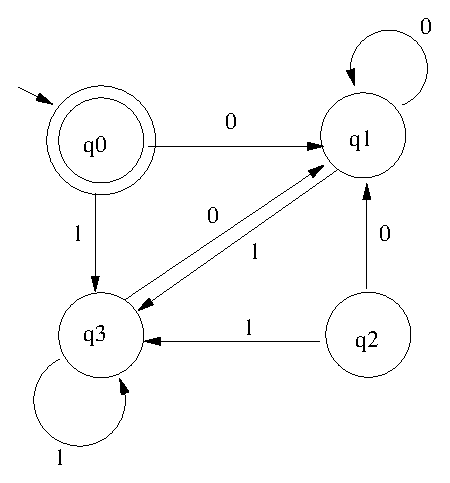
\includegraphics[width=8em]{fig.eps}}
        \caption{Exemplo de figura importada de um arquivo \texttt{.eps} e também exemplo de caption muito grande que ocupa mais de uma linha na Lista de~Figuras}
        \label{fig:ex1}
\end{figure}

% o `[h]' abaixo é um parâmetro opcional que sugere que o LaTeX coloque a
% figura exatamente neste ponto do texto. Somente preocupe-se com esse tipo
% de formatação quando o texto estiver completamente pronto (uma frase a mais
% pode fazer o LaTeX mudar completamente de idéia sobre onde colocar as
% figuras e tabelas)
%\begin{figure}[h]
\begin{figure}
        \begin{center}
        \setlength{\unitlength}{.1em}
        \begin{picture}(100,100)
                \put(20,20){\circle{20}}
                \put(20,20){\small\makebox(0,0){a}}
                \put(80,80){\circle{20}}
                \put(80,80){\small\makebox(0,0){b}}
                \put(28,28){\vector(1,1){44}}
        \end{picture}
        \end{center}
        \caption{Exemplo de figura desenhada com o environment \texttt{picture}.}
        \label{fig:ex2}
\end{figure}

Tabelas são construídas com praticamente os mesmos comandos. Lembre-se, porém, que o caption das tabelas deve ir em cima.

\subsection{Classificação dos etc.}

O formato adotado pela ABNT prevê apenas três níveis (capítulo, seção e subseção). Assim, \texttt{\char'134subsubsection} não é aconselhado.

\section{Sobre as referências bibliográficas}
Recomenda-se seriamente fazer uso do pacote \emph{bibabnt}, também disponibilizado na página do UTUG~\citeyearpar{UTUG:Homepage-01}. Esse pacote provê um estilo \textsc{BibTeX} para formatação de referências bibliográficas combinando normas da ABNT e do Instituto de Informática da UFRGS\@.

As seguintes referências são colocadas aqui a título de exemplo:
\cite{Andrews:CP-91, Silberschatz:OSC-3-91, Wilson:MME-01}.

A classe \emph{iiufrgs} faz uso do pacote \emph{natbib}. Esse pacote
disponibiliza diversos comandos alternativos para
citações. Os mais úteis para nós são o \texttt{\char'134citeyearpar},
que produz somente o ano (ex.~``[\ldots] são apresentados por Baker e
Smith~\citeyearpar{Baker:PP-96}.'') e o
\texttt{\char'134citep*}, que produz a citação com a lista
completa de autores (ex.~``[\ldots] na linguagem Panda~\citep*{Assenmacher:Panda-ECOOP93}.'')

% e aqui vai a parte principal
%
% \chapter{Estado da arte}
% \chapter{Mais estado da arte}
% \chapter{A minha contribuição}
% \chapter{Prova de que a minha contribuição é válida}
% \chapter{Conclusão}

% referencias
% aqui será usado o environment padrao `thebibliography'; porém, sugere-se
% seriamente o uso de BibTeX e do estilo abnt.bst (veja na página do
% UTUG)
%
% observe também o estilo meio estranho de alguns labels; isso é
% devido ao uso do pacote `natbib', que permite fazer citações de
% autores, ano, e diversas combinações desses
\begin{thebibliography}{este-parametro-nao-eh-usado-pelo-estilo-ABNT}

\bibitem[ANDREWS, 1991]{Andrews:CP-91} ANDREWS,
  G.~R\@. \textbf{Concurrent programming}: principles and
  practice. Redwood~City, USA: Benjamin/Cummings, 1991. 637p.
  
\bibitem[ASSENMACHER et~al.(1993)ASSENMACHER; BREITBACH; BUHLER;
  H{\"U}BSCH; SCHWARZ]{Assenmacher:Panda-ECOOP93} ASSENMACHER, H.;
  BREITBACH, T.; BUHLER, P.; H{\"U}BSCH, V.; SCHWARZ, R\@.
  Panda---supporting distributed programming in {C}++. In: EUROPEAN
  CONFERENCE ON OBJECT-ORIENTED PROGRAMMING, 7., 1993, Kaiserslautern,
  Germany. \textbf{Proceedings{\ldots}} Berlin: Springer-Verlag, 1993.
  p.361--383. (Lecture Notes in Computer Science, v.707).

\bibitem[BAKER; SMITH, 1996]{Baker:PP-96} BAKER, L.; SMITH,
  B.~J\@. \textbf{Parallel programming}. New~York: McGraw-Hill,
  1996. 381p.

\bibitem[CAROMEL; KLAUSER; VAYSSIERE, 1998]{Caromel:TSC-CPE-10-11-98}
  CAROMEL, D.; KLAUSER, W.; VAYSSIERE, J\@. Towards seamless computing
  and metacomputing in {J}ava.  \textbf{Concurrency: Practice and
  Experience}, West~Sussex, v.10, n.11--13, p.1043--1061,
  Sept./Nov.~1998.

\bibitem[FURMENTO; ROUDIER; SIEGEL, 1995]{Furmento:PDC-95} FURMENTO,
  N.; ROUDIER, Y.; SIEGEL, G\@. \textbf{Parall{\'e}lisme et
  distribution en {C}++}: une revue des langages existants. Valbonne,
  FR: I3S, Universit\'{e} de Nice Sophia-Antipolis, 1995. (RR~95-02).

\bibitem[INSTITUTE OF ELECTRICAL AND ELECTRONIC ENGINEERS,
  1995]{IEEE:Pthreads-95} INSTITUTE OF ELECTRICAL AND ELECTRONIC
  ENGINEERS\@. \textbf{Information Technology---Portable Operating
  System Interface (POSIX), Threads Extension [C Language]},
  \mbox{IEEE}~1003.1c-1995.  New~York, 1995.

\bibitem[SILBERSCHATZ; PETERSON; GALVIN, 1991]{Silberschatz:OSC-3-91}
  SILBERSCHATZ, A.; PETERSON, J.~L.; GALVIN, P.~B\@. \textbf{Operating
  system concepts}. 3.ed.  Reading, USA: Addison-Wesley, 1991. 696p.

\bibitem[UTUG(2001)UTUG]{UTUG:Homepage-01} UTUG\@. \textbf{Página do grupo
  de usuários {\TeX} da {UFRGS}}. Disponível em:
  $<$http://www.inf.ufrgs.br/utug$>$. Acesso em: maio 2001.

\bibitem[WILSON, 2001]{Wilson:MME-01} WILSON, P.~C\@. \textbf{Um
  método ótimo para o preparo de café em laboratório baseado na
  reciclagem de filtros}. 2001. 123p.  Disserta{\c{c}}{\~a}o (Mestrado
  em Ci{\^e}ncia da Computa{\c{c}}{\~a}o) --- Instituto de
  Inform{\'a}tica, Universidade Federal do Rio Grande do Sul,
  Porto~Alegre.

\end{thebibliography}

\end{document}
